\setchapterstyle{kao}
\setchapterpreamble[u]{\margintoc}
\chapter{First exercises with MicroPython on the ESP8266 microcontroller}
\labch{first_exercises}
This chapter covers a few concepts and skills you will need to work productively with microcontrollers. After some background, these are presented in the form of three exercises, in which you will learn: 
\begin{enumerate}
	\item How to connect your microcontroller to a platform called a \texttt{breadboard}, and how to use the microcontroller/breadboard combination to quickly assemble and troubleshoot circuits;
	\item How to use a microcontroller's electrical connections, called \texttt{General Purpose Input/Output} (\texttt{GPIO}) pins, to turn LEDs and other small devices on and off, and to respond to inputs like pressing a button; and,
	\item How to use a switch called a \texttt{relay} to turn on and off larger devices, that require too much current or voltage for your microcontroller to control directly.
\end{enumerate}

\vspace{2cm}
\begin{table}[h]
	\caption[\refch{first_exercises} materials]{\textbf{Materials you'll need\dots} 
		
		See Table \ref{tab:materials} for additional information.}
	\labtab{materials_1st_exercises}
\begin{center}
		\raggedright
	%\begin{tabular}{ c c c c }
	\begin{tabular}{ c r c}
		\hline
		Sections & item & link \\
		\hline
		\multirow{3}{4em}{\refsec{breadboards}} 
		%\multirow{2}{4em}{\vrefsec{breadboards}} 
		& breadboard & \ref{mat:bb} \\
		& ESP8266 ``Feather'' & \ref{mat:mc} \\
		& micro-USB cable & \ref{mat:usb_cbl} \\
		\hline
		\multirow{3}{4em}{\refsec{circuits}}  
		%\multirow{3}{4em}{\vrefsec{circuits}}  
		& male-male jumpers & \ref{mat:jmp_mm} \\ 
		& pliers & \ref{mat:plr} \\ 
		& resistors & \ref{mat:rsts} \\ 
		\hline
	\end{tabular}

\end{center}\end{table}
%\begin{margintable}[2.cm]
%	\caption[\refch{first_exercises} materials]{\textbf{Materials you'll need\dots} 
%		
%		See Table \ref{tab:materials} for additional information.}
%	\labtab{materials_1st_exercises}
%	\raggedright
%	%\begin{tabular}{ c c c c }
%	\begin{tabular}{ c r c}
%		\hline
%		Sections & item & link \\
%		\hline
%		\multirow{3}{4em}{\refsec{breadboards}} 
%		%\multirow{2}{4em}{\vrefsec{breadboards}} 
%		& breadboard & \ref{mat:bb} \\
%		& ESP8266 ``Feather'' & \ref{mat:mc} \\
%		& micro-USB cable & \ref{mat:usb_cbl} \\
%		\hline
%		\multirow{3}{4em}{\refsec{circuits}}  
%		%\multirow{3}{4em}{\vrefsec{circuits}}  
%		& male-male jumpers & \ref{mat:jmp_mm} \\ 
%		& pliers & \ref{mat:plr} \\ 
%		& resistors & \ref{mat:rsts} \\ 
%		\hline
%	\end{tabular}
%\end{margintable}


\section{Assembling circuits with microcontrollers and breadboards}
\labsec{breadboards}
For the purposes of this book, a \emph{circuit} is simply an assembly of wires and other electrical components intended to perform a useful task. 
Circuits need not be complicated --- a circuit consisting of only a battery, a wire, a switch and a light bulb is enough to make a flashlight, which can be very useful! 

Like this example, most circuits share a few common features, such as:
\begin{itemize}
	 \item A power source (or connections to attach one);
	 \item One or more components to regulate power, such as switches or resistors; and,
	 \item One or more components that convert electrical signals into physical effects (such as emitting light or turning a motor) or, alternatively, converting physical parameters into electrical signals (such as temperature or light sensors). 
\end{itemize}

In general, complicated circuits are built out of combinations of simpler ``sub-circuits''. Sub-circuits are parts of the overall circuit, that each have an identifiable and testable function. 
This \emph{modular} circuit design means that, if you start with simple circuits and understand them individually before they go into a complex circuit, the end result is easier to understand than if you contemplate an entire complex assembly at once. 
This sub-circuit based design is helpful for trouble-shooting as well.
%\sidenote[][*-12]{
	\begin{kaobox}[frametitle=Divide and conquer!]
		The key tactic of testing and debugging circuits is ``divide and conquer'': 
		If a complex circuit doesn't work (they usually don't, at first) try to divide it into two or more smaller, simpler sub-circuits.
		Then you can more easily assess which of these sub-circuits is causing the problem. 
		Often this has to be done multiple times, dividing a circuit into smaller and smaller parts until a problem is evident in one or more of them. 
		Having fixed the sub-circuit, work the other way by gradually reassembling larger subsets of components. 
		At the end of this process, the entire circuit will function as intended!
	\end{kaobox}
%}

For example, later in this Chapter, you will assemble a circuit enabling your microcontroller to ``snooze'' (slowly brighten and dim) an LED, in response to pressing a button. 
This circuit will comprise three  simpler sub-circuits, each responsible for a different task. 
One sub-circuit will distribute power to where it's needed in the circuit. 
Another will enable your microcontroller to detect when you press a button. 
The third will enable your microcontroller to turn power on and off to an LED. 
Because each of these sub-circuits has an identifiable, relatively simple function, each can be assembled and tested independently of the other sub-circuits. 
When all of these sub-circuits are working correctly, they will be linked together to form the complete circuit. 
This circuit will combine all the sub-circuits' functions to perform the intended task: suppling power to an LED regulated by the microcontroller in response to your pressing a button. 

Most of the exercises in this book will involve building, testing, troubleshooting and fixing one or more circuits. 
Initially this may feel unfamiliar.
After you have assembled your first few circuits, though, it will quickly come to feel much easier and more intuitive.

\subsection{Breadboard basics}
\begin{marginfigure}[-10.cm]
	\begin{center}
		\htmladdnormallink{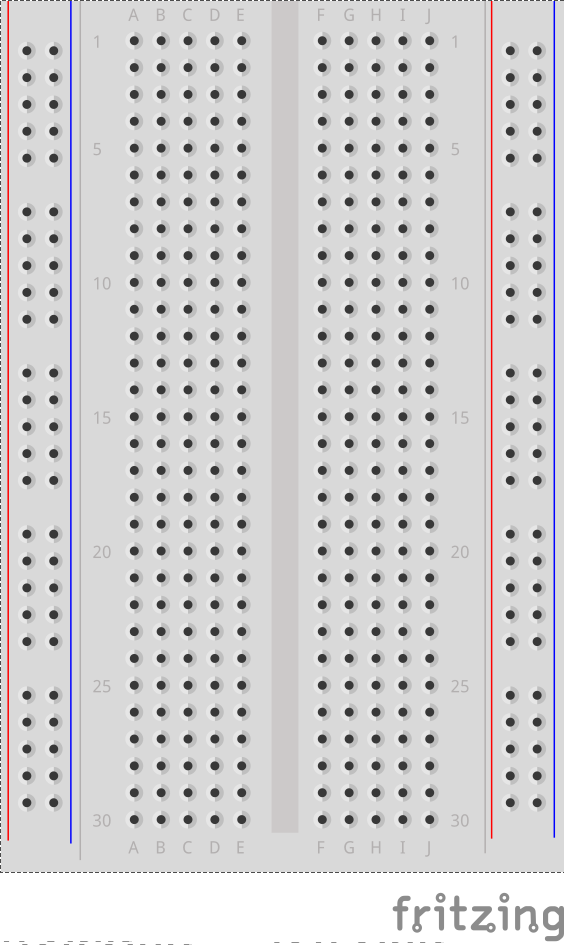
\includegraphics[width=\MFWn]{/home/dg/PublicSensors/Textbooks/IntroSensors/Fritzing/breadboard_bare.png}}{https://publicsensors.org/IntroSensors/Fritzing/breadboard_bare.png}
		\htmladdnormallink{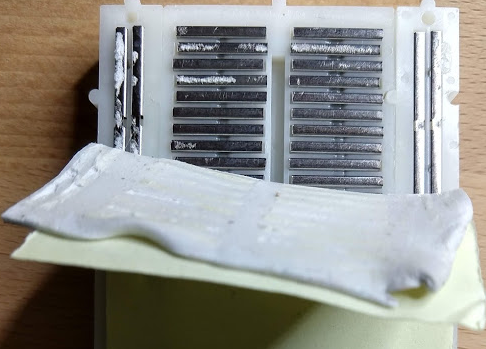
\includegraphics[width=\MFWn]{/home/dg/PublicSensors/Textbooks/IntroSensors/Images/breadboard_back1_crop.png}	}{https://publicsensors.org/IntroSensors/Images/breadboard_back1_crop.png}
		\caption[Breadboard front/back]{Breadboard front view, and back view with wires (partly) exposed.}
		\labfig{margin_breadboard}
	\end{center}
\end{marginfigure}
In the world of electronics, a \emph{breadboard} is a plastic or ceramic plate containing a large number of holes. 
Within the breadboard are hidden internal wires, connected in special patterns (\reffig{margin_breadboard}). 
When a wire is inserted into a breadboard hole, it makes an electrical connection with the hidden wires beneath, and is thereby connected to a specific set of other holes. %, \reffig{marginbb_schematic}). %\cref{margin_breadboard,marginbb_schematic}.  
The geometry of these holes and hidden wires is designed to make assembling and modifying circuits simple and fast, and to make it easy to understand connections among components. 

\emph{Prototyping} is the overall process of designing, assembling, correcting and enhancing new circuits. 
In prototyping, it is common (and usually harmless) to make small mistakes. 
Also, prototyping often involves some guesswork and iteration about \emph{layout} (e.g., which components should go next to which, to make wiring as compact and simple as possible).
The holes in breadboards are shaped so that wires (often called \emph{jumpers}\sidenote[][*-4]{\begin{kaobox}[backgroundcolor=\SNcolor,frametitlebackgroundcolor=\SNcolor,frametitle=Wire we using jumpers?]
	To make electrical connections on a breadboard, we use wires called ``jumpers''. 
	Jumpers are mostly covered with insulation, to avoid accidental connections (``short circuits''). 
	However, the last few millimeters on both ends are \emph{stripped} (the insulation is removed) so that they fit into the breadboard. 
	You can buy jumpers in several different forms, or make them yourself out of thin solid core wire. 
	In our lab, we have lots of old ethernet cable, with 8 strands of wire that is perfect for making jumpers. 
	Store-bought jumpers seem much more expensive than they ought to be, so we encourage you to make your own whenever possible.\end{kaobox}}) can be easily inserted and removed from them.
When you find a mistake or want to change the circuit design, it is straightforward to add wires, or to pull existing wires out of their present holes and move them into new holes.
Breadboards are useful, among other reasons, because they help make this process of circuit prototyping more straightforward and efficient
%\sidenote[][*-0]{
%	For sensors intended to function in the environment, sometimes it is sufficient to use a circuit built on a breadboard. 
%	Other times, however, circuits must be made as small as possible (e.g. to fit into a waterproof housing), resistant to vibrations, etc.
%	In these cases, it may helpful to use soldered connections on a \htmladdnormallink{``stripboard''}{https://en.wikipedia.org/wiki/Stripboard} or a Printed Circuit Board (PCB). 
%	This is usually done after a fully functional prototype is developed on a breadboard.
%	For instructions on how to make your own PCBs, see \refch{PCB_design}.
%}
%\begin{marginfigure}[-0.cm]
%	\begin{center}
%			\htmladdnormallink{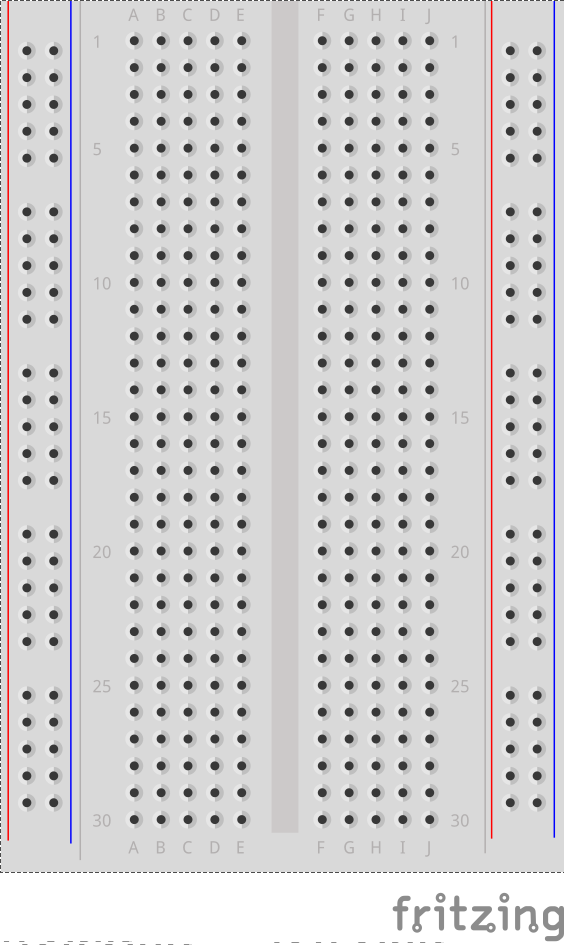
\includegraphics[width=\MFWn]{/home/dg/PublicSensors/Textbooks/IntroSensors/Fritzing/breadboard_bare.png}}{https://publicsensors.org/IntroSensors/Fritzing/breadboard_bare.png}
%			\htmladdnormallink{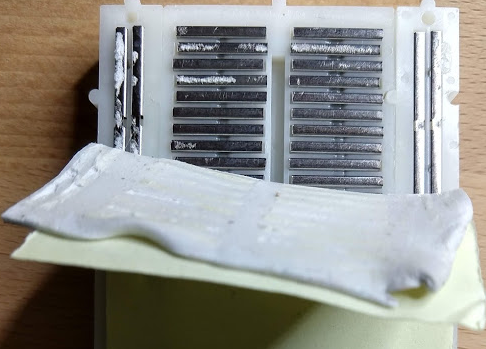
\includegraphics[width=\MFWn]{/home/dg/PublicSensors/Textbooks/IntroSensors/Images/breadboard_back1_crop.png}	}{https://publicsensors.org/IntroSensors/Images/breadboard_back1_crop.png}
%		\caption[Breadboard front/back]{Breadboard front view, and back view with wires (partly) exposed.}
%		\labfig{margin_breadboard}
%	\end{center}
%\end{marginfigure}

%In comparison to tweaking a circuit that is soldered together, working with breadboards is much faster and easier! 
%After a little experience, it will become almost automatic to follow connections on a breadboard to tell how a circuit is laid out and what it does. 

The holes on breadboards are laid out in \emph{rows} and \emph{columns}. 
The interior section of a typical breadboard has two rectangular blocks of holes, with five holes in each row on each side of a ``gutter''. 
In these interior sections, the five holes within one row on either side of the gutter are connected by a hidden wire. 
However, holes in one row are not connected to holes in other rows. 
Furthermore, holes on one side of the gutter are not connected to the holes on the other side (\reffig{marginbb_schematic}).

The breadboard's hidden connections mean that any set of wires inserted into holes in the same row on the same side of the gutter are connected. 
On the other hand, any wires inserted into holes in different rows, or in the same row but on opposite sides of the gutter, are \emph{insulated} from each other (not connected). 
This straightforward geometry makes it easy to make it easy to understand the layout of an existing circuit, or to build a new one. 
 
Alongside the interior blocks of holes, most breadboards have paired columns of holes. 
Unlike the interior holes, these exterior sets of holes are connected in columns but not in rows. 
These exterior columns of holes, sometimes called \emph{rails}, are usually reserved for purposes such as supplying power to components distributed across the breadboard. 

\begin{marginfigure}[-4 cm]
	\begin{center}
		\htmladdnormallink{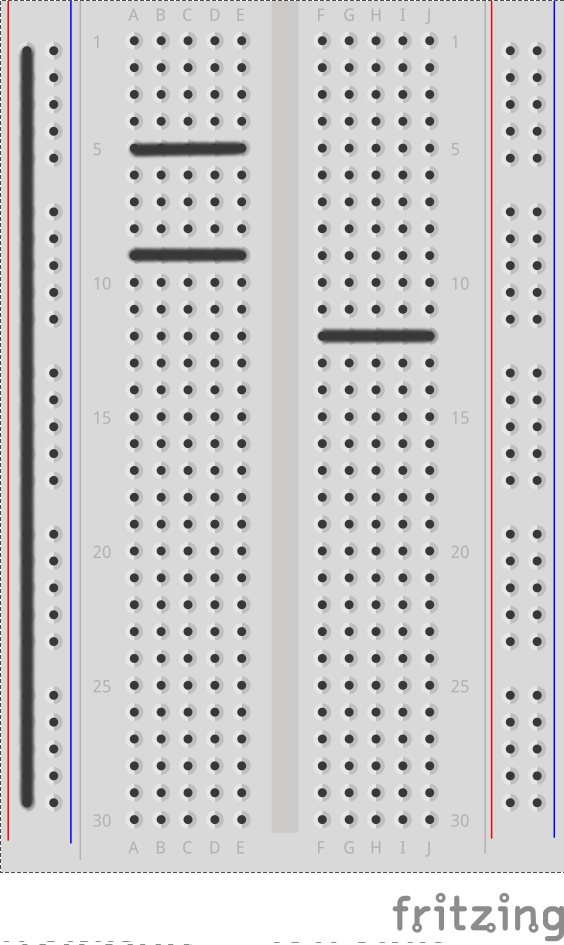
\includegraphics[width=\MFW]{/home/dg/PublicSensors/Textbooks/IntroSensors/Fritzing/breadboard_connections.png}}{https://publicsensors.org/IntroSensors/Fritzing/breadboard_connections.png}
		\caption[Breadboard connections schematic]{An illustration of the connections provided by hidden wires in a typical breadboard. The five holes in each interior row are connected, as indicated by the horizontal black lines. The gray vertical line is the ``gutter'' --- holes on opposite sides of the gutter are \underline{not} connected. Holes are also connected in exterior columns (called ``rails''), indicated here by the vertical black line.}
		\labfig{marginbb_schematic}
	\end{center}
\end{marginfigure}

One of the rails on each side is often marked with a ``+'' or a red line (\reffig{marginbb_schematic}). 
This column is usually attached to the positive terminal of a battery or power supply.
The corresponding rail might be marked with a ``-'' or a blue line.
This column is usually attached to the negative or \emph{ground} terminal. 
These rails make it possible to supply power and ground connections to components anywhere on the breadboard, using only very short wire connections that are visually neat and have minimal crossings. 
Circuits laid out with short, neat connections are usually easier to assemble and troubleshoot than equivalent circuits laid out with long loopy or crisscrossing wires.

Breadboards come in a wide range of different sizes and shapes, suitable for different kinds of projects. 
Smaller breadboards may have only a few rows, and may lack power and ground rails. 
Larger breadboards may be composed of several subunits, each of which has independent interior sections and rails.  
Despite differences in size, however, the same basic geometry of hidden wires connecting interior rows and (if present) exterior columns applies to all of these breadboard configurations.

%\section{Meet your microcontroller}
%\labsec{microcontrollers}
%Now it's time to start working with your microcontroller. 
%To begin with, a little background about microcontrollers: 
%A \emph{microcontroller} is a device with a processing unit that can run codes and other instructions, and with external connections (called \emph{pins}) to transmit electrical inputs and outputs. 
%There exist many types of microprocessors, which vary by overall size, power requirements, capabilities to input and output different kinds of electrical signals, onboard communication hardware like WiFi or USB connectors, and the types of code or instructions they accept. 
%
%This textbook focuses on microprocessors that use instructions written in \htmladdnormallink{MicroPython}{https://micropython.org/}, a subset of the \htmladdnormallink{Python}{https://www.python.org} programming language.
%MicroPython is a recent invention, and a great improvement for learning about, building and using environmental sensors.
%Because MicroPython-based microcontrollers are automatically interactive
%\sidenote[][*-6]{Like Python, MicroPython runs in an interactive session. 
%	This session goes by the  technical-sounding name ``Read-Evaluate-Print-Loop'', or \emph{REPL}. Despite this name, REPL is a very intuitive interface. 
%	REPL simply means that, in a MicroPython (or Python) session, you type commands, which are then executed, and the results are then displayed.
%}
%, they are good platforms to develop and debug codes to collect data from environmental sensors.  
%Python itself is a powerful and easy to learn language for scientific computing on desktops and laptops. If you already know some Python, you can apply that knowledge to working with MicroPython-based microcontrollers. If you're new to Python, then by learning MicroPython you will simultaneously learn how to use Python for many other tasks. In fact, many of the exercises in this book combine acquiring data from sensors, and analyzing or plotting those data on a computer, using the same coding language!
%  
%\subsubsection{Adafruit's Feather HUZZAH ESP8266 microcontroller}
%
%\begin{marginfigure}[-18cm]
%	\begin{center}
%			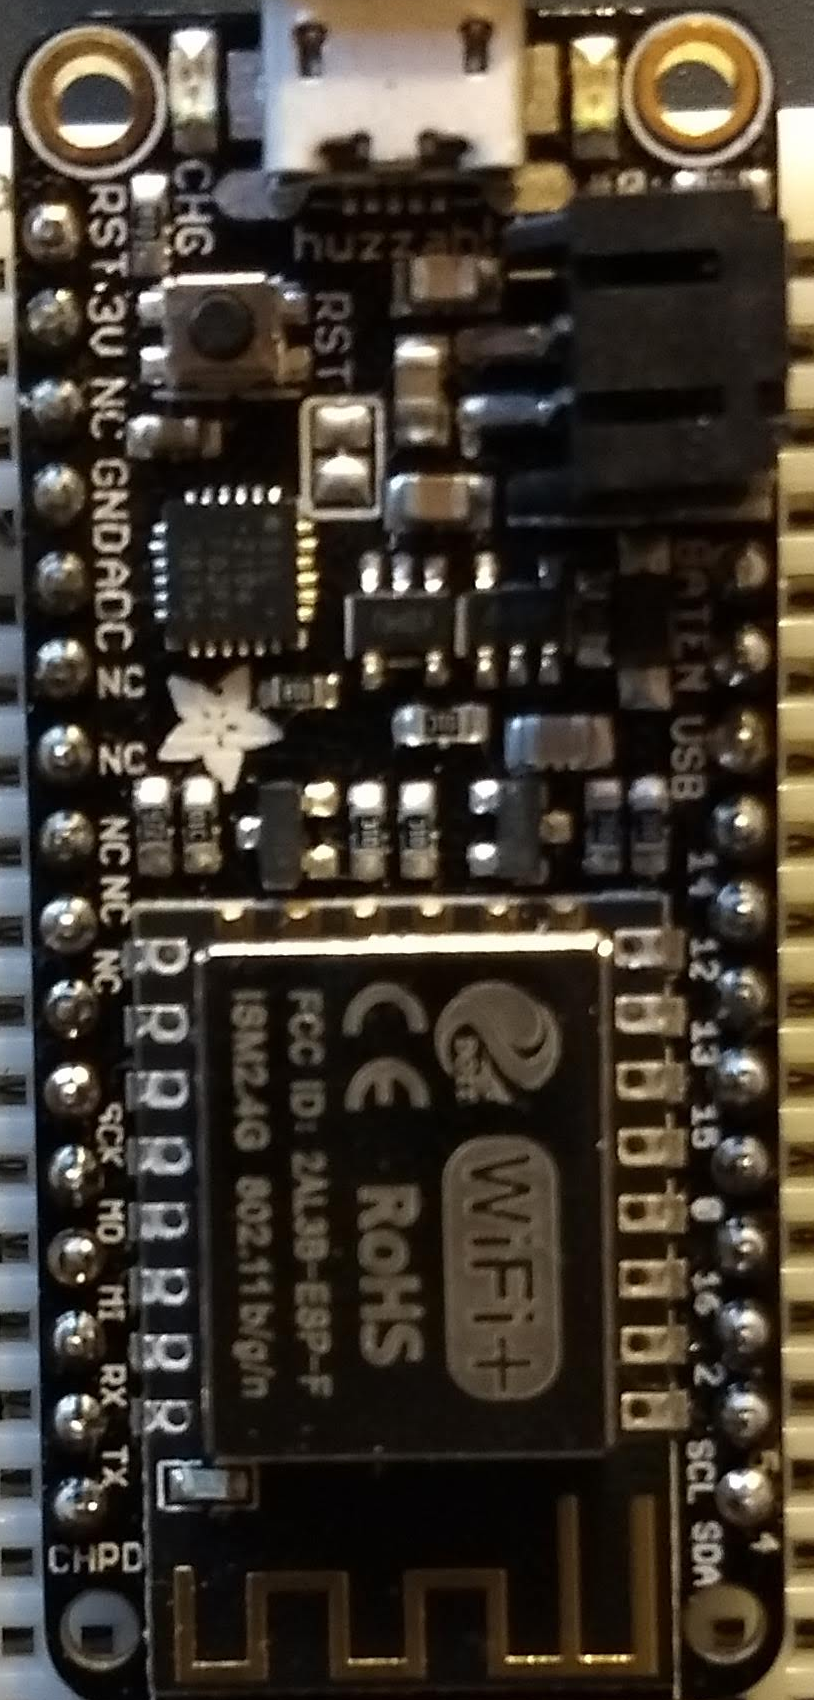
\includegraphics[height=6cm]{/home/dg/PublicSensors/Textbooks/IntroSensors/Images/ESP8266feather_top.png}
%		\caption[ESP8266 feather microcontroller]{A ESP8266 Feather microcontroller.}
%		\labfig{margin_esp8266}
%	\end{center}
%\end{marginfigure}
%
%For examples in this book, we will use Adafruit's Feather HUZZAH ESP8266 microcontroller. 
%It is small, has built-in wifi, uses relatively little power, and is low cost for its capabilities. 
%The core ESP8266 microcontroller was originally intended to be placed in ``smart'' lightbulbs.\sidenote[][*+8]{See e.g. \htmladdnormallink{Tinnkerman's light bulb hacks}{https://tinkerman.cat/post/yet-another-wifi-light-bulb/} for some fun examples in which the ESP8266 microcontroller is reprogrammed in place within a smart light bulb.}
%Very large scale production for this purpose has made this microcontroller inexpensive, which also makes it a good choice for putting sensors in often-harsh environments.
%
%Note that the exercises in this book can be successfully completed using other microcontrollers. 
%We focus here on the Feather ESP8266 because it is one of the microcontrollers officially supported by \htmladdnormallink{MicroPython}{https://http://micropython.org/}, and because Adafruit provides good documentation and support for it.
%Other manufacturers also make microcontroller boards based on the ESP8266. 
%Many of these will work in essentially the same way. 
%Boards using other processors also can work, but may require modifying details such as pin numbers. 
%The \htmladdnormallink{MicroPython}{https://http://micropython.org/} website is the best reference if you are considering using alternative microprocessor boards for the activities in this book.
%
%
%A close-up view of the ESP8266 Feather (\reffig{margin_esp8266}) shows the key features we will use to create functional environmental sensors.
%\marginnote[-0cm]{
%	The documents \htmladdnormallink{adafruit-huzzah-esp8266-breakout.pdf}{https://cdn-learn.adafruit.com/downloads/pdf/adafruit-huzzah-esp8266-breakout.pdf} and  \htmladdnormallink{adafruit-feather-huzzah-esp8266.pdf}{https://cdn-learn.adafruit.com/downloads/pdf/adafruit-feather-huzzah-esp8266.pdf} are the best overall resources for information about the Adafruit Huzzah Breakout and Feather versions of the ESP8266 microcontroller. 
%	Please download the document for your microcontroller for future reference about specifications, pin definitions, voltage tolerances, etc.
%}
%The core microcontroller is the rectangular component near the bottom.
%The zigzag line below it is a built-in WiFi antenna. 
%At the top is a connector for a microUSB cable, used to communicate with the Feather. 
%Plugging a USB cable into this connector and into your computer automatically supplies power to the microcontroller. 
%It also automatically supplies a connection for communicating with the microcontroller -- see \refch{connect} for instructions on how to use USB to communicate with your microcontroller.
%
%Below and to the left of the USB connector is a button, labelled ``\texttt{RST}''. 
%This is a reset button, used occasionally to halt a run-away code or reboot a hung or malfunctioning microcontroller (normally we will do this via software, so we rarely need to use the \texttt{RST} button).
%At the four corners are holes for mounting screws. 
%Along the right and left edges are soldered pins, which are spaced to fit into a breadboard, and which have different capabilities to transmit electrical signals to and from the microcontroller. 
%These pins have labels alongside (sometimes a little above or below) that identify the pin. 
%We will learn more about how to use these pins in the next section. 


%
%\begin{lstlisting}
%	\begin{marginfigure}
%		\includegraphics{/home/dg/PublicSensors/Textbooks/IntroSensors/Images/IMG_20181205_082817686.jpg}
%		\caption[ESP8266 feather microcontroller on breadboard, too]{Breadboard with ESP8266 feather, again.}
%		\labfig{esp8266brd}
%	\end{marginfigure}
%\end{lstlisting}

%\sidenote[][*-0]{
%\begin{kaobox}[frametitle=Beyond breaboarding \dots]
\begin{kaobox}[frametitle=Board with circuit design \dots]
	For sensors intended to function in the environment, sometimes it is sufficient to use a circuit built on a breadboard. 
	Other times, however, circuits must be made as small as possible (e.g. to fit into a waterproof housing), resistant to vibrations, etc.
	In these cases, it may helpful to use soldered connections on a \htmladdnormallink{``stripboard''}{https://en.wikipedia.org/wiki/Stripboard} or a Printed Circuit Board (PCB). 
	This is usually done after a fully functional prototype is developed on a breadboard.
	For instructions on how to make your own PCBs, see \refch{PCB_design}.
\end{kaobox}%}

\subsection{Using General Purpose Input/Output (GPIO) pins}
Microcontrollers are useful because they are able to transmit and receive electrical signals to and from other devices.
These signals are passed through connections called \texttt{General Purpose Input/Output} pins, usually abbreviated as \texttt{GPIOs}.  

Important things to know about GPIOs on the ESP8266 are:
\begin{itemize}
	\item[$\bullet$] Pins labeled with numbers (0, 2, 4, 5, 12, 13, 14, 15 and 16) are GPIOs.
	\item[$\bullet$] GPIOs can be set by software commands to work as either \emph{input} or \emph{output} pins (but not both simultaneously).
	 \begin{itemize}
		\item[$\circ$] In output mode, a GPIO is set by the microcontroller to take on a specific voltage. 
		\item[$\circ$] Output mode is typically used when the microcontroller needs to \underline{send} a signal.
		\item[$\circ$] In input mode, a GPIO is set by the microcontroller to detect the voltage supplied to the pin by another component. 
		\item[$\circ$] Input mode is typically used when the microcontroller needs to \underline{receive} a signal.
	\end{itemize}
	\item[$\bullet$] These GPIOs are \emph{digital}. This means that these pins can only take one of two values:
	 \begin{itemize}
	 	\item[$\circ$] 1, or ``high'', corresponding to a voltage $\ge 3.3$ \texttt{volts}\sidenote[][*0]{\begin{kaobox}[backgroundcolor=\SNcolor,frametitlebackgroundcolor=\SNcolor,frametitle=What's your limit?]Note that the \texttt{3.3 volt} threshold applies to the ESP8266, and to many other microcontrollers. 
	 		Some have different thresholds, though, so if you're using a different microcontroller it's a good idea to check.\end{kaobox}}; or,
	 	\item[$\circ$] 0, or ``low'', corresponding to a voltage $< 3.3$ \texttt{volts}.
	\end{itemize}
	\item There is one other pin on the ESP8266, labeled \texttt{ADC} (for Analog to Digital Conversion), that can measure any voltage between 0  and 1 \texttt{volts}. \refch{circuits_intro} explains how to use the \texttt{ADC} pin to measure battery level, get readings from analog environmental sensors, \etc
%	this threshold is )\texttt{GND} or 0 volts; or, 
%	 	, above a specific threshold (for the ESP8266, this threshold is ); or,	 
\end{itemize} 
With this background, it's time to learn what GPIOs can do by building some simple circuits!

\subsubsection{GPIOs as outputs}
Your first activity with your microcontroller will be to use GPIO pins as \emph{outputs}. 
This means that you will use MicroPython commands to set the on/off state of specific pins. 
Using GPIOs in their other mode, as \emph{inputs}, will come in the next section.

The ESP8266 Feather has two built-in LEDs, that are connected inside the microcontroller board to two of the GPIO pins. 
\begin{itemize}
	\item[$\circ$] Pin 0 is connected to a red LED. 
	\item[$\circ$] Pin 2 is connected to a blue LED.
\end{itemize}
Because these LEDs are already present without need for external connections, and because they make visible the state of the pins they connect with, they make a good starting point for learning to use GPIOs.

\subsubsection{\howto Turn on/off the on-board LEDs}
To control the red LED, you will use the \lstinline{Pin} method from Micropython’s \lstinline{machine} package.
\begin{marginfigure}[-2cm]
	\htmladdnormallink{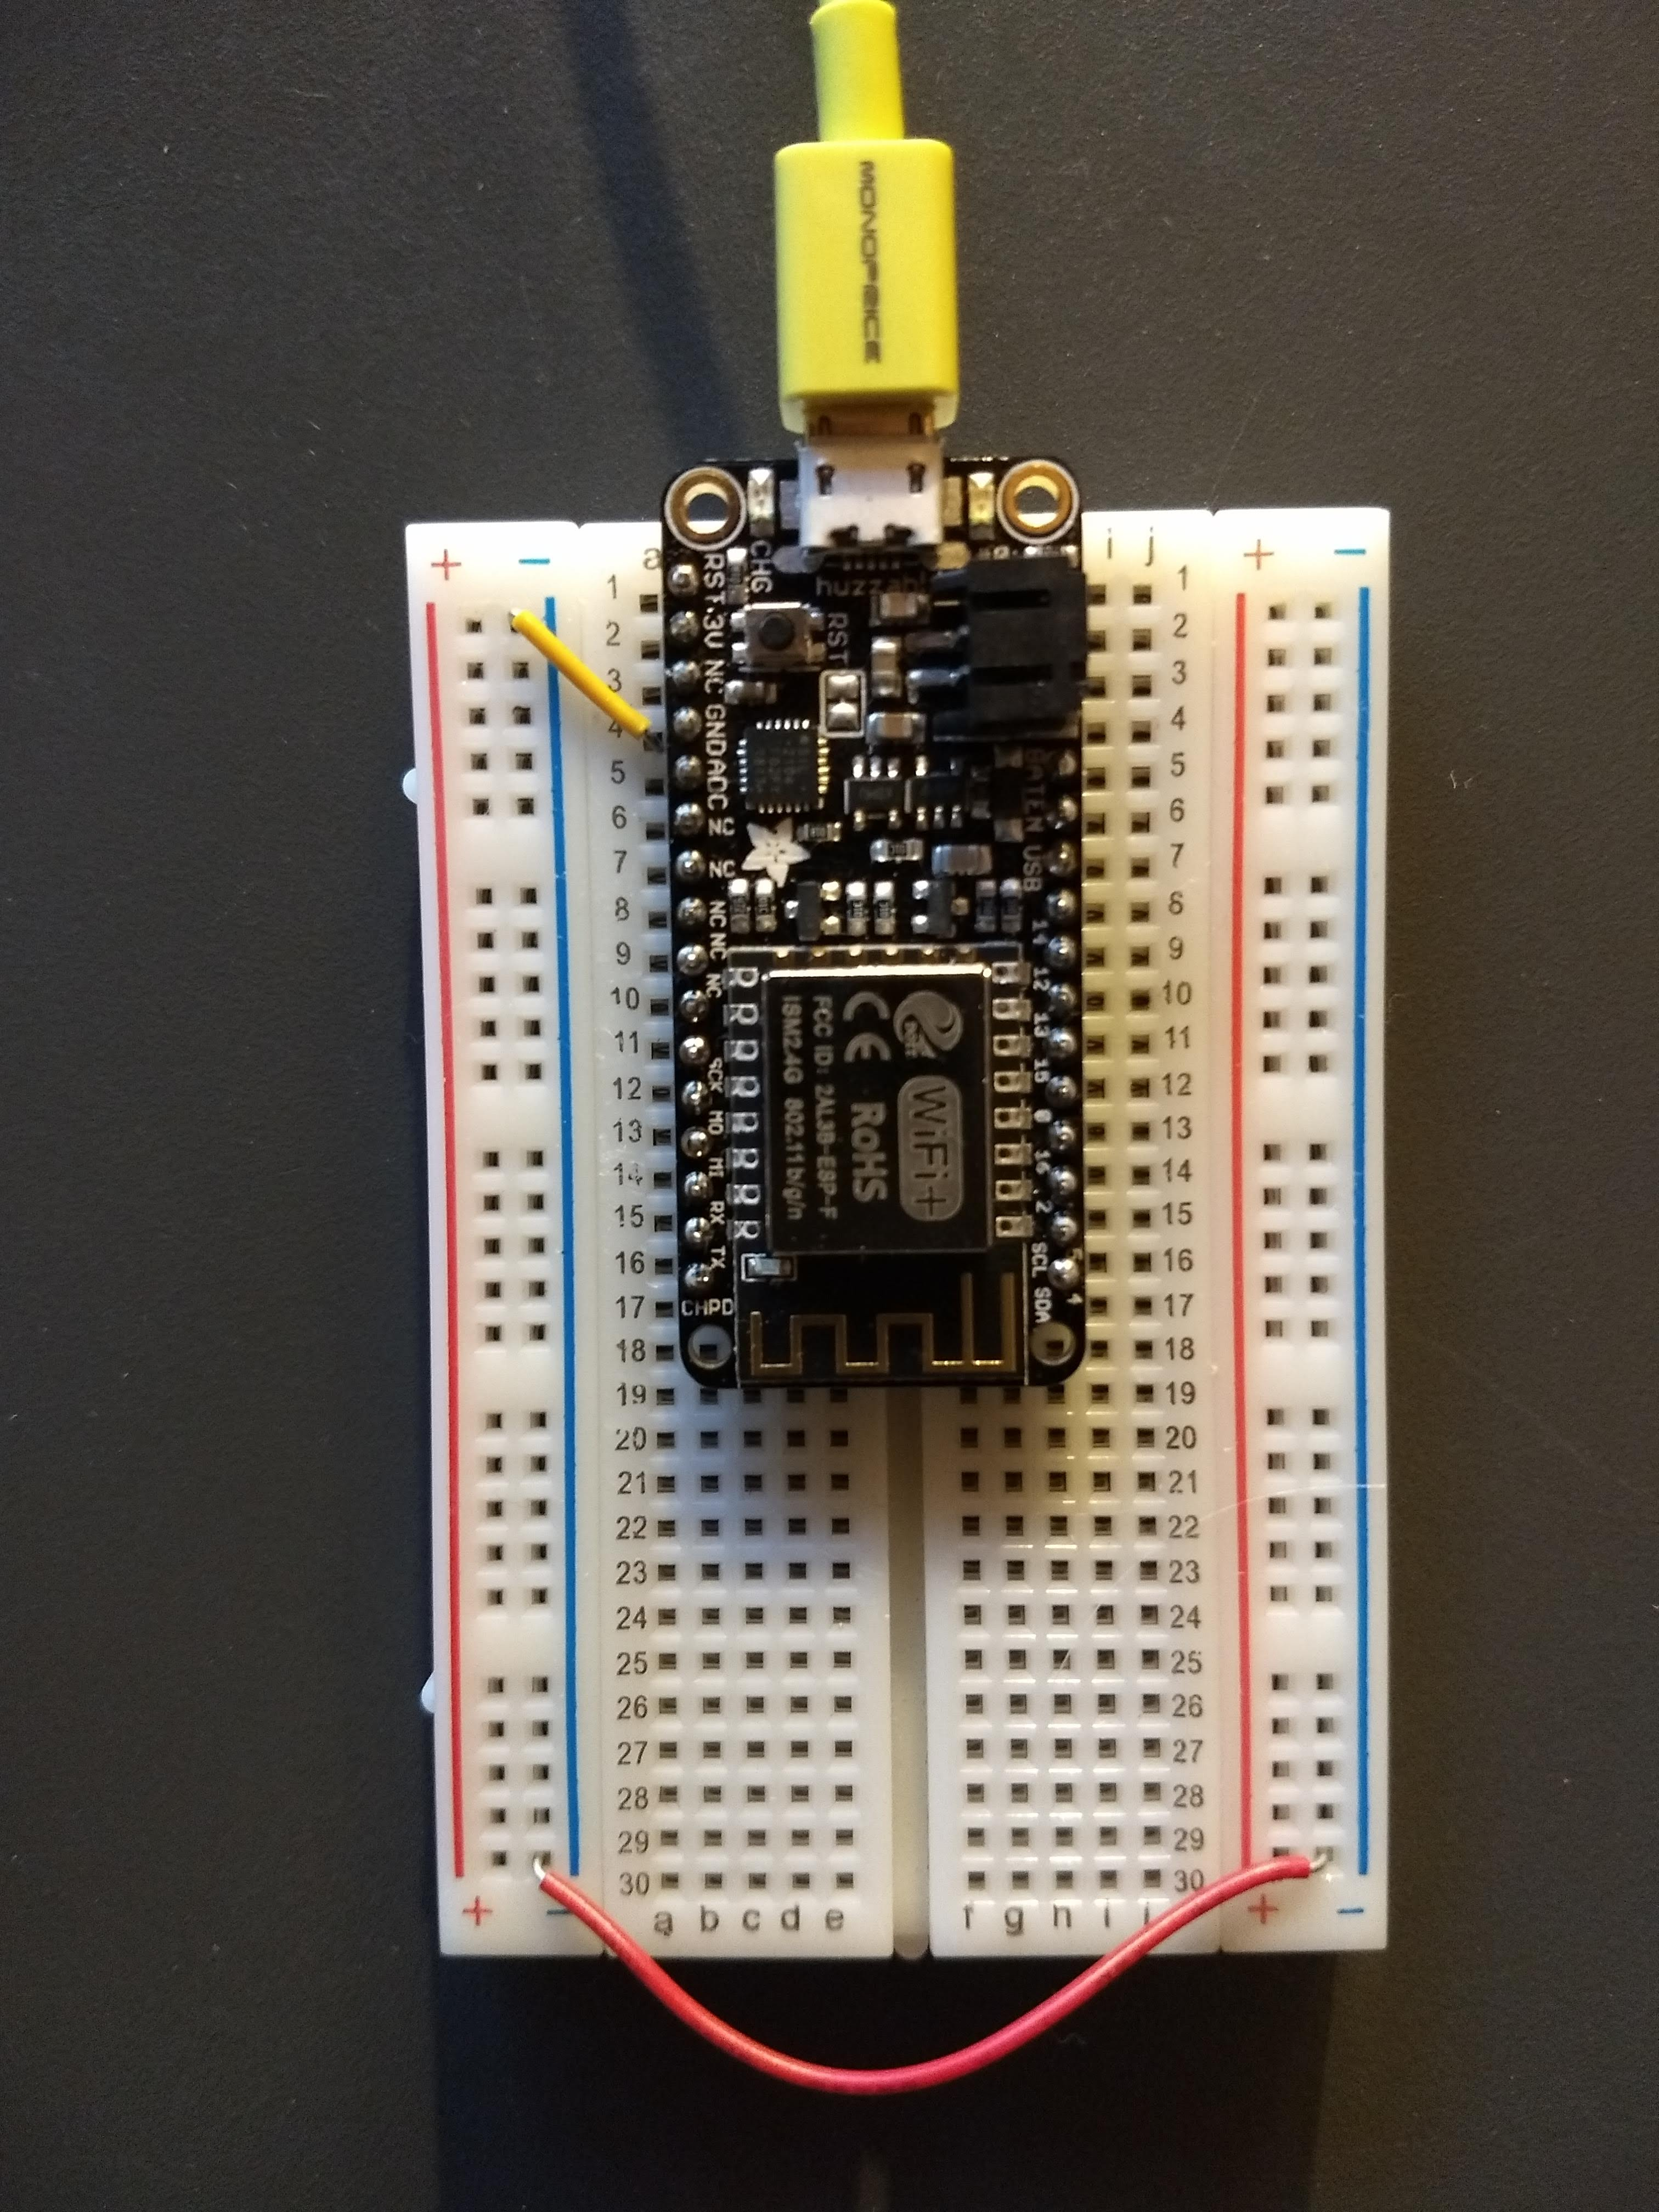
\includegraphics[width=\MFW]{/home/dg/PublicSensors/Textbooks/IntroSensors/Images/breadboard_ESP8266feather.jpg}}{https://publicsensors.org/IntroSensors/Images/breadboard_ESP8266feather.jpg}
	\caption[ESP8266 feather microcontroller on breadboard]{Breadboard with ESP8266 feather.}
	\labfig{margin_breadboard_esp8266}
\end{marginfigure}

%\sidenote{
%	In this section, we assume you have already established communications with your microcontroller. 
%	If you have not yet done that, please see %\refpart{conns} %
%	\refch{connect} %\refch{usb_connect} and \refch{wifi_connect} 
%	for instructions before proceeding.}
\begin{enumerate}
	\item \textbf{Mount your microcontroller on a breadboard and connect a USB cable, as shown in \reffig{margin_breadboard_esp8266}.} 
	
	\begin{itemize}
		\item[$\circ$] Note that the USB connector is facing upwards, off the board, to make it easy to reach. 
		\item[$\circ$] The first row of pins projecting below the board are inserted into the breadboard in the top row of breadboard holes. 
		
		This is to leave as many rows below the ESP8266 as possible accessible for circuit-building. 
	
		\item[$\circ$] The microcontroller fits onto the breadboard either with one open column of holes on the left and two on the right, or with two on the left and one on the right. 
		
		\smallskip
		For this set of exercises, either position is OK.
	\end{itemize} 
%is mounted on a On your ESP8266, each of the numbered pins inserting into your breadboard is a GPIO. Each of these is available for transmitting and receiving signals, although some of these pins also have other functions.

	\item \textbf{Open a \texttt{REPL} session}
	
	\item \textbf{Import the \texttt{Pin} class}:%\sidenote[][*-0]{In this book, we will use this format to indicate code to be entered typed into a REPL session on your microcontroller, or to be put into a file to be run on your microcontroller or laptop.}:
\begin{lstlisting}[language=Python]
from machine import Pin 
\end{lstlisting}	

	\item \textbf{Create a \texttt{Pin} object pointing to \texttt{GPIO 0}, setting that pin into output mode}:
\begin{lstlisting}[language=Python]
pin0 = Pin(0, Pin.OUT) 
\end{lstlisting}	
	
	\begin{itemize}
		\item[$\circ$] In this Python statement, \texttt{pin0} is the name of the object to be created. 
		This name could in general be almost anything, but it's a good idea to make names as informative as possible. 
		In this case, ``pin'' will remind us that it's a \texttt{Pin} object, and the ``0'' reminds us that it points to \texttt{GPIO 0}.
	
%	\smallskip
	
	\item[$\circ$] Inside the call to the \texttt{Pin} method, the \texttt{0} indicates the object will be attached to \texttt{GPIO 0}, and \texttt{Pin.OUT} sets that GPIO into output mode.
	\end{itemize}
 
	\item \textbf{Use the \texttt{pin0} object to query or set the state of this pin, by entering the follows commands}:
\begin{lstlisting}[language=Python]
pin0.value()  # returns the present state of GPIO 0
pin0.value(1) # sets state of GPIO 0 to 1, or ``on''
pin0.value()  # returns the present state of GPIO 0
pin0.value(0) # sets state of GPIO 0 to 0, or ``off''
pin0.value() # returns the present state of GPIO 0
\end{lstlisting}
	Note that \texttt{pin0.value(1)} causes \texttt{GPIO 0} to be set at \texttt{3.3 volts}.
	\texttt{pin0.value(0)} causes GPIO 0 to be set at \texttt{0 volts}.
	Which of these corresponds to the red LED turning on? Is that what you expected? 
	
	\item \textbf{Control pin state with } \lstinline{on} \textbf{and} \lstinline{off}.
	The pin object also allows you to use \lstinline{pin0.on()} and \lstinline{pin0.off()} to set the state of a GPIO in output mode. 
	Try this and verify that you can toggle the LED on and off.
	Keep in mind, though, that this notation can be confusing. 
	For example, in some circuits, invoking \lstinline{pin0.on()} turns an attached device  off, and \textit{vice versa}. 
	To avoid ambiguity, we usually stick with the \lstinline{pin0.value()} method when using GPIOs.
	
	\item \textbf{Repeat the steps above, but this time create an object pointing to \texttt{GPIO 2}.}
	
	\emph{Things to think about \dots}
	\begin{itemize}
		\item What is an informative name for this new object? 
		\item What is the behavior of the microcontroller when you execute these commands?
	\end{itemize}
\end{enumerate}

%%\begin{kaobox}[frametitle=Milestones Overview]
%%	\begin{itemize}
%%		\item 
%\marginnote[-5cm]{
%		\loadMilestone{mlst:ov} % load milestone with tags id: mlst:ov}%	\end{itemize}
%}%\end{kaobox}
%
%%{\color{orange} \rule{\linewidth}{0.5mm} }
%%\begin{kaobox}[frametitle=Using GPIOs as outputs]
%%	\begin{itemize}
%%		\item[$\Box$] 
%\marginnote[0cm]{
%		\loadMilestone{mlst:02a} % load milestone with tags id: mlst:02
%}%	\end{itemize}
%%\end{kaobox}
%%{\color{orange} \rule{\linewidth}{0.5mm} }


\loadMilestone{mlst:02a} % load milestone with tags id: mlst:02

%\marginnote[0cm]{
	\begin{kaobox}[frametitle=Some MicroPython shortcuts...] \label{copy_paste}
	Micropython has shortcuts that can save you lots of typing. 
	\begin{itemize}
	\item[$\bullet$] Hitting the up arrow ($\uparrow$) parses through previous commands so you can edit and re-execute them.
	\item[$\bullet$] To paste in a block of formatted python code (e.g. from a python editor on your laptop), type 
\begin{lstlisting}[language=Python]
<ctrl>-e
[pasted python code]
<ctrl>-d
\end{lstlisting}
	As an example, copy the code you used to control the red LED, and paste it into an editor on your laptop. 
	Now, use the \texttt{<ctrl>-e}/\texttt{<ctrl>-d} sequence to paste this code to the ESP8266. 
	The pasted code will be executed when you type the \texttt{<ctrl>-d}.

	\item  \texttt{<ctrl>-d} by itself (that is, not preceeded by \texttt{<ctrl>-e}) reboots the ESP8266! 
	This causes the Micropython session to “forget” all the previous commands and clear all its memory. 
	In Python, it is not possible to import a library twice. 
	So, if you need to re-import a corrected or modified code, rebooting in this way may be necessary. 
	\end{itemize}
	\end{kaobox}
%}

\section{Creating circuits on a breadboard}
\labsec{circuits}
Now you're ready to use your microcontroller/breadboard combination to experiment with some circuits. 
If you've never used a breadboard, or if it’s been awhile since you did, a good way to start is to create a circuit that ``snoozes'' an external LED by making it gradually get brighter and dimmer.
In this section, we will follow a typical prototyping process by laying out this circuit in the form of several sub-circuits. 
We'll assemble each of these sub-circuits in turn, testing and (if necessary) debugging each before proceeding to the next. 
When they are working correctly, we'll integrate them into the emerging circuit to give it new capabilities.  

\subsection{Distributing power across the breadboard}
The first sub-circuit we'll construct will connect the positive and negative rails, so that power and ground connections are easily accessible from all parts of the breadboard.
\begin{marginfigure}[-0cm]
	\begin{center}
		\htmladdnormallink{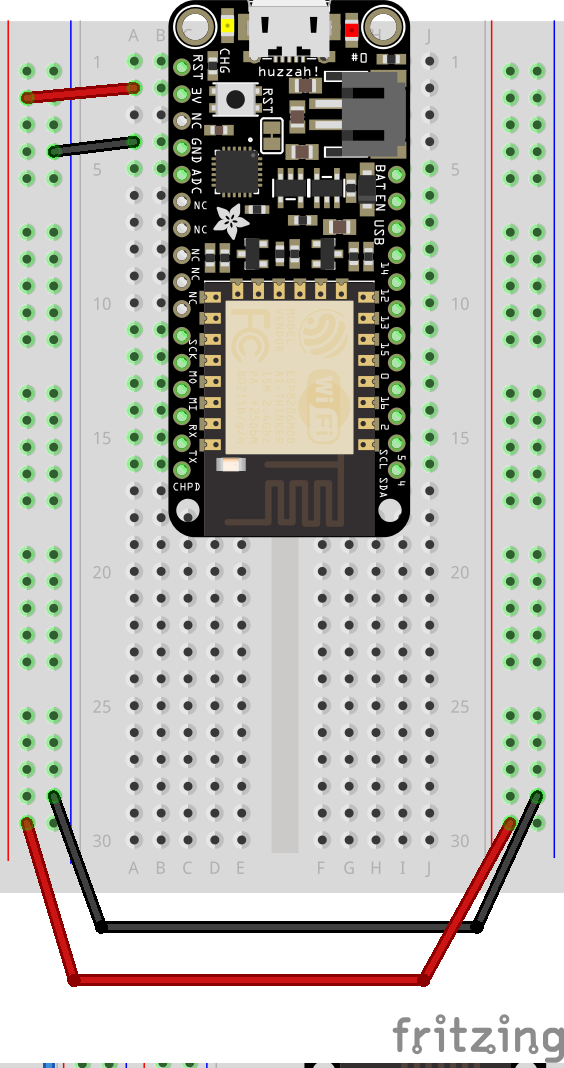
\includegraphics[width=\MFW]{/home/dg/PublicSensors/Textbooks/IntroSensors/Fritzing/feather_rails.png}}{https://publicsensors.org/IntroSensors/Fritzing/feather_rails.png}
		\caption[Power/ground rails connection schematic]{Typical layout for connecting power and ground rails to a Feather microcontroller.}
		\labfig{feather_rails}
	\end{center}
\end{marginfigure}

\subsubsection{\howto Construct a power distribution sub-circuit}
\begin{enumerate}
	\item \textbf{Disconnect your ESP8266 from the USB cable}.
	
	It is often wise to turn off power to the microcontroller while you assemble circuits. 
	Otherwise, misplacing a jumper, or even briefly brushing it against the microcontroller or another component, can cause a short circuit and permanently damage your microcontroller! 
 	
 	Because the USB cable automatically supplies power, the only way to turn off power to the microcontroller is to disconnect the USB cable.
	When you're done assembling the circuit, check that the connections are as you intended before connecting again to USB power.  
	
	\item \textbf{Use a jumper to connect the \texttt{GND} pin on the ESP8266 to the negative (blue) rail}.
	
	To complete this step, note the pin labeled \texttt{GND} (for ``ground'', or \texttt{0 volts}) on the upper left side of the Feather in \reffig{margin_esp8266}. 
	One end of the jumper should be inserted into an open hole in the same row as the \texttt{GND} pin. 
	The other end should be inserted somewhere in the exterior column of holes immediately to the left (see \reffig{feather_rails}).
	
	\item \textbf{Use a longer jumper to connect the bottom hole in the left side negative rail to the bottom hole on the right side negative (blue) rail}. 
	
	Your jumpers should now look something like the black lines in \reffig{margin_breadboard_esp8266}. 
	In this configuration, any wire inserted into the negative rail on either side will be automatically connected to ground (\texttt{0 volts)}.
	
	\item \textbf{Connect the pin marked \texttt{3V} on the ESP8266 to the positive (red) power rail.}
	
	The \texttt{3V} pin, on the upper left side of the Feather, supplies a constant 3.3 volts from a voltage regulator (there is not enough room on the board to write the second decimal place!).	
%	The \texttt{USB} pin, located on the upper right side of the microcontroller, is connected internally to the USB power supply. 
%	USB power is always supplied at \texttt{+5 volts}. 
%	Use another jumper to connect an empty hole in the same row as the \texttt{USB} pin to any hole in the right side positive rail.
	
	\item \textbf{Use a longer jumper to connect the bottom hole in the left side positive rail to the bottom hole on the right side positive rail}. 
	
	Now, any wire inserted into the positive rail on either side will be automatically connected to \texttt{3.3 volts}.
	
	%The power rails are the two outermost sets of pins, arranged in columns running the length of the breadboard. These make electrical power easily available to devices connected to the power rails.
	\item \textbf{Check your circuit}.

	Make sure that, in the circuit you assembled: the left positive rail is connected to the \texttt{3V} pin, the right positive rail is connected to the left positive rail, the left negative rail is connected to the \texttt{GND} pin, and the right negative rail is connected to the left negative rail.
	
	\emph{Confirm that at no point does a jumper connect the positive part of the circuit directly to a negative part of the circuit.}

	\item \textbf{Plug your USB cable back into the microcontroller}.
	
	Use a multimeter to test your circuit, making sure it works correctly. 
	An easy way to do this is to use insert one end of a male-male jumper into one of the positive rails. 
	Insert one end of \textbf{another} male-male jumper into one of the negative rails. 
	Now, use the multimeter to test the voltage difference between the free ends of the two jumpers.
	\sidenote[][*-4]{\begin{kaobox}[backgroundcolor=\SNcolor,frametitlebackgroundcolor=\SNcolor,frametitle=CAREFUL!]Make sure not to connect the positive and negative rails directly together --- for example by brushing the leads of the multimeter to each other while they are touching the rails. This would cause a short circuit that could damage your microcontroller!\end{kaobox}}
	
\end{enumerate}
\loadMilestone{mlst:02b} % load milestone with tags id: mlst:02b

\subsection{GPIO as inputs: Responding to button pushes}
One of the most useful things a GPIO does is let you control your microcontroller through external devices like switches. 
For example, in an environmental sensor, you might want to turn sampling on and off with a button switch, have nearby motion trigger a camera, or count rotations of a propeller to measure wind speed. All of these involve using GPIOs as inputs. 

As a first step, you will assemble a sub-circuit enabling the microcontroller to respond to button presses. 
\sidenote[][*-12]{\begin{kaobox}[backgroundcolor=\SNcolor,frametitlebackgroundcolor=\SNcolor,frametitle=Button it up!]
	The type of switch used in this circuit is called a \emph{momentary} switch. 
	``Momentary'' means the switch will connect two pins while the button is being pressed, and immediately disconnect them when the button is released. 
	Many other types of switches are available for different functions. 
	For example, some switches \emph{toggle}: they form a connection when a button is pressed, and don't disconnect until the next time the button is pressed. Other types of switches are turned off by light, magnetic fields, or electrical signals instead of buttons.
\end{kaobox}}A typical sub-circuit enabling a microcontroller to respond to button pushes is illustrated in \reffig{feather_switch}. 
This sub-circuit will require a button switch and two jumpers, and a few lines of code. 
When this sub-circuit works properly, you'll incorporate it into the other components of the circuit so that a button push starts and stops LED snoozing. 



Like many button switches, this one has four pins. 
This is mostly for mechanical support, to keep the pins from breaking or pulling out too easily.
Two pairs of these pins are connected to each other, so there are really just two independent sets of pins that are connected and disconnected by button presses.

Notice that the pins are not equally spaced. 
The different spacing is to help you orient the button correctly.
 
On two opposite edges, pins are spaced to skip over \emph{three} holes on a breadboard. 
We will call these the \emph{wide} sides.
On this type of button, the wide side pins are always internally connected to each other. \sidenote[][*-10]{\begin{kaobox}[backgroundcolor=\SNcolor,frametitlebackgroundcolor=\SNcolor,frametitle=Button orientation]
	In most breadboard layouts, a button's wide side pins are placed in the same row on the same side of the gutter as in \reffig{feather_switch}. 
	Occasionally, though, the wide side pins are placed on opposite sides of the gutter, in which case they act as a jumper connecting adjacent rows across the gutter. 
	In this configuration, pressing the button connects all four breadboard rows (two on each side of the gutter)!\end{kaobox}}

On the perpendicular edges, pins are spaced to skip over \emph{two} holes on a breadboard. 
We will call these the \emph{narrow} sides.
The narrow side pins are insulated from each other, unless the button is pushed. 
While the button is being held down, a connection is made across the narrow sides.
When the button is released, the narrow side pins are again insulated from each other.

\subsubsection{\howto Assemble a button switch sub-circuit}
\begin{enumerate}
	\item  \textbf{Connect your button to the breadboard.}
	
	As shown in \reffig{feather_switch}, make sure the wide sides are aligned with a row. As usual, the exact rows in which the button is placed are not critical. However, it's a good idea to place the button reasonably close to the bottom of the microcontroller, so there is enough room below to assemble other sub-circuits.
	
\begin{marginfigure}[-0cm]
	\begin{center}
		\htmladdnormallink{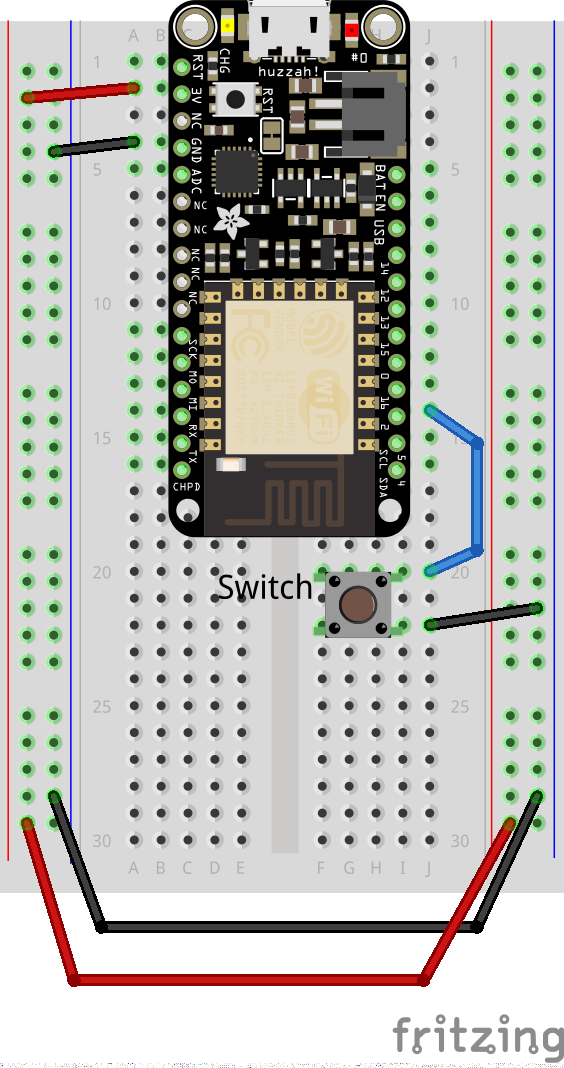
\includegraphics[width=\MFW]{/home/dg/PublicSensors/Textbooks/IntroSensors/Fritzing/feather_switch.png}}{https://publicsensors.org/IntroSensors/Fritzing/feather_switch.png}
		\caption[Button connections schematic]{An illustration of the layout for connecting a button switch to an input GPIO on the Feather. Notice the orientation of the button: The more widely spaced pins orient along rows, and the more narrowly spaced pins orient along columns.}
		\labfig{feather_switch}
	\end{center}
\end{marginfigure}

	\item  \textbf{Jumper one wide side pin pair to the negative rail.}
	
	Because all the holes in the negative rail are connected to each other, any of them will work for our purposes. This means we're free to choose a hole that makes our sub-circuit compact and neat, and out of the way of other sub-circuits. 

	\item  \textbf{Jumper the other wide side pin pair to \texttt{Pin 2}.}
	
	Any of the numbered pins can act as input GPIOs. By choosing \texttt{Pin 2}, we will be able to see the effect of our button via the on-board red LED.
	
%\end{enumerate}
%That's it for the hardware. 

%Now we need to import the Pin method, define \texttt{GPIO 2} as an input pin, and test whether our button sub-circuit works as intended:
	\item \textbf{Import the Pin method, and define \texttt{GPIO 2} as an input pin.}
\begin{lstlisting}[language=Python]
from machine import Pin 
pin2 = Pin(2, Pin.IN,pull=Pin.PULL_UP) 
\end{lstlisting}	
	In the call to the \texttt{Pin} method, the \texttt{pull=Pin.PULL\_UP} tells the microcontroller that its default value should be ``high'' (\texttt{3.3V}). When the button is pressed, \texttt{GPIO 2} is connected (through the switch and negative rail) to \texttt{GND} (\texttt{0V}). This changes \texttt{GPIO 2} from ``high'' to ``low''.

%\begin{itemize}
	\item \textbf{Test the sub-circuit.}
	
	When you press the button, you should see a change in the state of the blue LED indicating \texttt{GPIO 2} changed from ``high'' to ``low''. 
	When you release the button, it should revert to its default state. 
	
	You can directly query the state of \texttt{GPIO 2} with the command
\begin{lstlisting}[language=Python]
pin2.value() 
\end{lstlisting}	
	Try it, to confirm that \texttt{GPIO 2} turns from value 1 (\texttt{3.3V}) to value 0 (\texttt{0V}) when you press the button, and reverts to value 1 when you release it.
	
\end{enumerate}
Does this happen? 
If so, congratulations, you've made a functional button input! 
If not, examine each of the component placements on the breadboard, and each line of MicroPython code you executed. 
When you find the difference between what you did and what you meant to do, the sub-circuit will be fixed.
\loadMilestone{mlst:02c} % load milestone with tags id: mlst:02c

\subsection{Acting reflexively: GPIO \texttt{interrupts} and \texttt{handlers}}
Now that you have a button that conveys a signal to your microcontroller, how can you use it to perform a useful function? 
One approach would be to have a code that continually checks whether a button is being pressed or not. 
However, this wastes a lot of processing power, and besides is cumbersome to incorporate into environmental sensor codes. 

Like most modern microcontrollers, \texttt{ESP8266}s can be programmed to have ``reflexes'', which cause them to automatically perform a task when a specific GPIO changes between its ``high'' and ``low'' states. 
These reflexes are called \emph{interrupts}, because (with some exceptions) they can be triggered even when the microcontroller is busy running a MicroPython script to perform another task. 

There are two steps to defining a GPIO \texttt{interrupt}:
\begin{enumerate}
	\item Instruct the microcontroller what you want to happen as a response when a GPIO shifts from ``high'' to ``low'', or from ``low'' to ``high'' (these can have different responses). 
	These instructions takes the form of a Python method, called a \emph{handler}. 
	
	\item Program one of the GPIOs to execute that \texttt{handler} when its state changes.

\end{enumerate}
These steps are best explained with an example. 

\subsubsection{\howto Program an interrupt responding to button presses}
Suppose we would like to set up our microcontroller so that, when we press the button, it \emph{toggles} the red LED (that is, it alternately switches \texttt{Pin 0} on and off). \verb|button_interrupt.py| is an example of code giving this behavior using our button sub-circuit:
\begin{enumerate}
	\item \textbf{Download the} \lstinline{button_interrupt.py} \textbf{python script, and copy it onto your microcontroller.}
	\lstinputlisting[language=Python,label=ButtonInterrupt,caption={\htmladdnormallink{\texttt{button\textunderscore interrupt.py}}{https://publicsensors.org/IntroSensors/Codes/button_interrupt.py}: A Micropython script to toggle the state of GPIO 2 when GPIO 0 changes state.}]{Codes/button_interrupt.py}
	\item \textbf{In a \texttt{REPL} session, import the module:}
\begin{lstlisting}[language=Python]
import buttonInterrupt
\end{lstlisting}	
	Now, in addition to the direct action of the button (changing the state of the blue LED), it also triggers an \texttt{interrupt} that changes the state of the red LED.
	\item \textbf{Optionally, replace the} \lstinline{pin2.irq} \textbf{command by uncommenting one of the alternatives below it.}
		
	\texttt{GPIO} \texttt{interrupts} respond to pin state transitions high$\rightarrow$low as different types of events from low$\rightarrow$high transitions.
	In coding an \texttt{interrupt}, you can specify responses to either or both of these transitions.
	
	\smallskip
	How does your circuit behave if you use \lstinline{trigger=Pin.IRQ_FALLING|Pin.IRQ_RISING} to define your \texttt{interrupt}, so it responds to both high$\rightarrow$low and low$\rightarrow$high state changes?
\end{enumerate}
\loadMilestone{mlst:02d} % load milestone with tags id: mlst:02b



\subsection{Controlling external devices using your microcontroller.}
Now that you have some familiarity with \texttt{GPIO}s, and have the power distribution sub-circuit set up on your breadboard, you are ready to build a sub-circuit to power and control an external LED. 
Because this sub-circuit is a little more complex, we will construct it in parts --- ``sub-sub-circuits'' --- that are simpler to assemble, test, and if necessary debug.
There are three of these parts: powering an external LED; installing a relay to control the LED; and, programming an interrupt to switch the relay on and off.
\subsubsection{\howto Power an external LED}
\labsec{ext_led}
We'll begin by wiring an LED into the existing components on your breadboard. 
\reffig{feather_switch_LED} illustrates the layout of the sub-circuit you're about to build.
As usual, there is some flexibility about exactly which hole and which row a wire is placed. 
However, it's a good idea to look over \reffig{feather_switch_relay_LED} to see where additional components will be placed, and to leave space for those.
Placing components similarly to \reffig{feather_switch_LED} is one way to do that. 
\begin{marginfigure}[-10cm]
	\begin{center}
		\htmladdnormallink{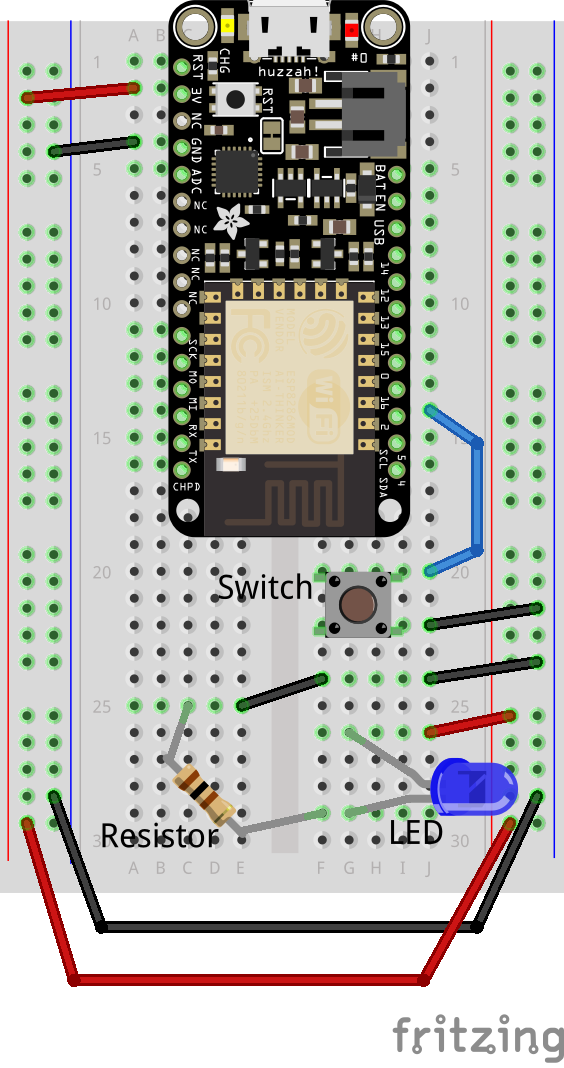
\includegraphics[width=\MFW]{/home/dg/PublicSensors/Textbooks/IntroSensors/Fritzing/feather_switch_LED.png}}{https://publicsensors.org/IntroSensors/Fritzing/feather_switch_LED.png}
		\caption[Button connections schematic]{An illustration of the layout for an external LED. }
		\labfig{feather_switch_LED}
	\end{center}
\end{marginfigure}


\begin{enumerate}
	\item \textbf{Connect a jumper from the negative rail on the right side of the breadboard, to the rightmost hole in a row slightly below the button.}
	\item \textbf{Connect a jumper from the leftmost hole in this row, across the gutter to one row lower.}
	
	This jumper placement will make it easy to substitute a relay for the jumper later on. 
	\item \textbf{Using a 100 Ohm resistor\sidenote[][*-5]{
			\begin{kaobox}[backgroundcolor=\SNcolor,frametitlebackgroundcolor=\SNcolor,frametitle=Pi\`ece de r\'esistance]
				Depending on which type of LED you use, you may need to modify the value of this resistor. 
				In \refch{circuits_intro}, you will learn how to calculate appropriate resistor values if you use a different type of LED than the one suggested here (though many types are close enough to work with the suggested resistor). 
				In the meantime, you can use an online   \htmladdnormallink{LED Resistor Calculator}{http://www.ohmslawcalculator.com/led-resistor-calculator} to figure out which resistor you need.
			\end{kaobox}
		}: Connect one wire to the left end of that jumper, and the other end into a row somewhere on the right side of the gutter.} 
	
	It does not matter which end of the resistor you start with, because resistors function the same way in either direction. 
	The exact row you connect to on the right side of the gutter also doesn't matter --- you are free to use any row as long as it is empty, and it's reasonably convenient to connect with jumpers to the other components in the circuit. 
	If you are unsure, pick a row and see if it works. 
	If connections later seem awkward or confusing, it's easy to move components to different rows to make the circuit smaller and neater.
	
	
	
	\item \textbf{Connect your LED into your circuit.}
	
	On your LED, notice that the two wires are of different lengths. The longer wire on an LED is always the positive side, and the shorter wire is the negative side. Connect the negative (shorter) LED wire to another hole in the same row as the resistor. Now connect the positive (longer) wire on the LED to an empty row. 
	
	\item \textbf{Connect the row with the positive wire from the LED to any hole in the positive (red) power rail.}
	
	\item \textbf{Check your circuit}.
	
	Confirm that, in the circuit you assembled: the LED is electrically connected on its positive terminal to 3.3 \texttt{volts} from the ESP8266; and, on its negative side, the LED is connected to the resistor, which in turn is connected to GND.
	
	\item \textbf{Plug your USB cable back into the microcontroller}.
\end{enumerate}
Does the LED light up? If so --- congratulations, you’ve made a working circuit! 
If not, check carefully that each of the connections was exactly what you intended, and that the positive and negative wires on the LED are in the appropriate holes. 
It’s easy to make small mistakes, but usually also easy to correct them!
\loadMilestone{mlst:02e} % load milestone with tags id: mlst:02e


\subsubsection{\howto Switch the LED with a relay}

Having built a circuit to power an external LED, you are now ready to enhance that circuit to enable your ESP8266 to control the LED.
To accomplish this, you will create a circuit using a \emph{relay}.

A relay is a switch that is controlled by an electrical signal. 
Relays help overcome a basic limitation of microcontrollers: they can supply only low levels of voltage and current. 
How, then, can a microcontroller control a device that requires large voltages or currents?
By switching on and off an external power supply (which may be high voltage or current), relays enable your ESP8266 to control external devices, even ones that require far more current or voltage than the microcontroller can supply directly.

The relay in the circuit you build in this example will control only a small device (an LED).
However, the same circuit configuration with a larger power supply and more robust relay could be used to control large equipment like winches, pumps, light banks, etc. that use large amounts of current or high voltages. 


\begin{marginfigure}[0cm]
	\begin{center}
		\htmladdnormallink{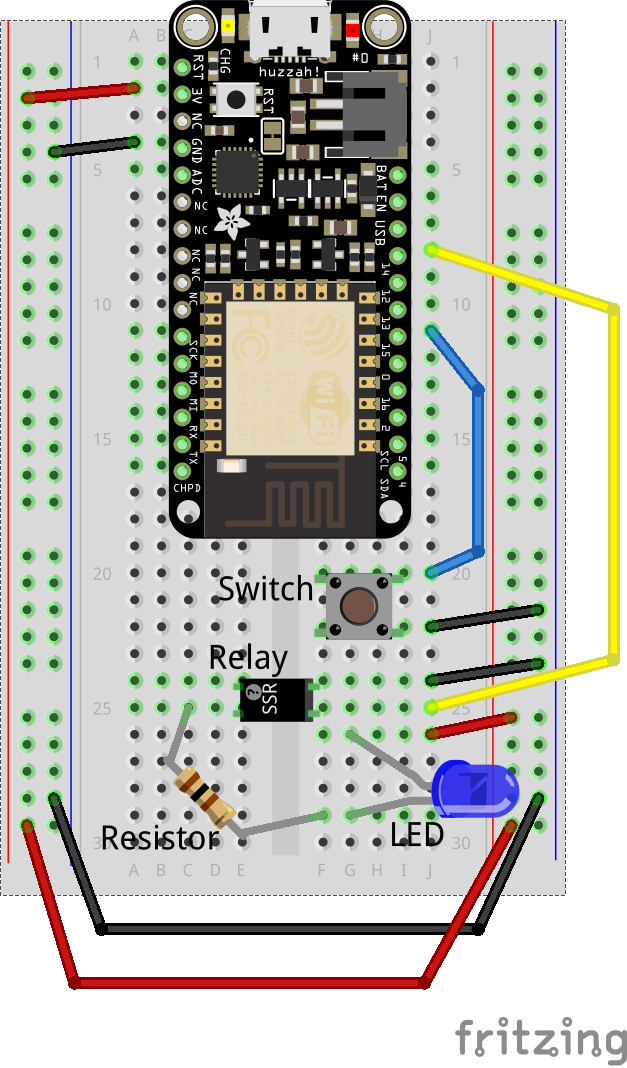
\includegraphics[width=\MFW]{/home/dg/PublicSensors/Textbooks/IntroSensors/Fritzing/feather_switch_relay_LED.png}}{https://publicsensors.org/IntroSensors/Fritzing/feather_switch_relay_LED.png}
		\caption[Button connections schematic]{An example of layout for the relay-LED sub-circuit }
		\labfig{feather_switch_relay_LED}
	\end{center}
\end{marginfigure}

%The figure is: \reffig{feather_switch_relay_LED}

%\begin{marginfigure}[5cm]
%	\includegraphics{/home/dg/PublicSensors/Textbooks/IntroSensors/Images/LEDrelay_circuitESP8266feather.jpg}
%	\caption[ESP8266 LED relay circuit]{A circuit in which an ESP8266 Feather microcontroller switches an LED using a relay.}
%	\labfig{margin_LEDrelay_esp8266}
%\end{marginfigure}

As you build your circuit, refer to \reffig{feather_switch_relay_LED} %\reffig{margin_LEDrelay_esp8266}
 for guidance:

\begin{enumerate}
	\item \textbf{Disconnect your ESP8266 from the USB cable}.

	\item \textbf{Remove the jumper spanning across the gutter}. 
	
	\item \textbf{In its place, insert a relay into your breadboard, as shown in the illustration}.
	Make sure that: 
	\begin{itemize}
		\item[$\circ$] The relay spans across the ``gutter''; and
		\item[$\circ$] The relay is oriented so that the writing is rightside up (with the tops of letters closest to the ESP8266).
		
		This may be easier with the aid of a magnifying glass. Note the pins are different on the two sides of the relay, making it easier to tell which side is which.
	\end{itemize}
	
	\item \textbf{Connect the upper right pin on the relay to the negative (blue) power rail.}
	
	\item \textbf{Connect the lower right pin on the relay to the hole next to pin 14 on the ESP8266.} 
	
	This is the GPIO pin you will use to control the relay (note the pin is a little above the label).
	
%	\item \textbf{Connect one wire of a 100 Ohm resistor to the upper left pin on the relay. Put the other end into a row somewhere below the relay (again, it does not matter exactly which one).}
%	
%	\item \textbf{Put the negative (short) wire of your LED into another hole in the same row as the resistor, on the same side of the gutter.}
%	
%	\item \textbf{Now, connect the positive (long) wire on the LED to the positive (red) power rail.}

	\item \textbf{Check your circuit.}	
	
	In particular, make sure that, on the left side of the gutter, the resistor is connected to the left side of the relay.

	\item \textbf{Plug your USB cable back into the microcontroller}.
\end{enumerate}

That’s it for the hardware! Now we need to do the software:

\begin{enumerate}[resume]
	\item \textbf{Initialize GPIO 14 as you did for pins 0 and 2 before, and toggle its value:}
\begin{lstlisting}[language=Python]
from machine import Pin
p14 = Pin(14, Pin.OUT)
p14.value()
p14.value(1)
p14.value()
p14.value(0)
\end{lstlisting}
\end{enumerate}
Did the GPIO control the external LED? If so – well done, you’ve used a relay to control a device! 
If not, look things over and see if you can find a flaw in the assembly of your circuit or the Python commands to control it.
\loadMilestone{mlst:02f} % load milestone with tags id: mlst:02f

\subsection{Fine control using Pulse Width Modulation}
The GPIO pins on your ESP8266 (and many other microcontrollers) are digital, meaning they can output only two values --- high and low. 
That's great for devices that need to be fully on or fully off. 
However, in many cases it’s useful to have an intermediate. 
One way to approach this is known as \htmladdnormallink{Pulse Width Modulation}{https://en.wikipedia.org/wiki/Pulse-width_modulation} (\texttt{PWM}). 
In \texttt{PWM}, the GPIO output is switched between ``on'' and ``off'' states very quickly (e.g. 1000 times per second), but the total fraction of time spend in the ``on'' state is varied gradually between 0 and 1. 
This is a close approximation to being able to continuously adjust pin states between on and off.

Let’s test what this does with our LED circuit. 
This test does not require any hardware modifications. 
We just need to redefine GPIO 14 in the code, to be a \texttt{PWM} pin instead of a simple digital output pin.

\subsubsection{\howto Snoozing an external LED}
%To keep things simple, do a soft reboot by typing \texttt{<ctrl>-d}. 
\begin{enumerate}
	\item \textbf{Create a PWM object attached to \texttt{GPIO 14}, and test it to make sure it regulates the LED:}
	\begin{lstlisting}[language=Python]
	from machine import Pin, PWM  # import the necessary modules
	pwm14 = PWM(Pin(14))      # create PWM object for GPIO 14
	pwm14.freq()             # get current frequency
	pwm14.freq(1000)         # set frequency
	pwm14.duty()             # get current duty cycle
	pwm14.duty(400)          # set duty cycle
	\end{lstlisting}
	Did the intensity of the LED change? 
	If so, you've succeeded!
	If not, check the code and the wiring to see where the mistake is.
	\smallskip
	Try changing the \texttt{PWM} parameters to make the LED brighter and fainter: 
	\begin{lstlisting}[language=Python]
	pwm14.duty(700)  # set a higher duty cycle
	pwm14.duty(100)  # set a lower duty cycle
	\end{lstlisting}
	\item \textbf{Using the \texttt{<ctrl>-e}/\texttt{<ctrl>-d} technique (or by downloading for the link), copy and execute the following code on your microcontroller:}
	\lstinputlisting[language=Python,label=SnoozeLED,caption={\htmladdnormallink{\texttt{snoozeLED.py}}{https://publicsensors.org/IntroSensors/Codes/snoozeLED.py}: A Micropython script to ``snooze'' an LED regulated by \texttt{GPIO 14}, using Pulse Width Modulation.}]{Codes/snoozeLED.py}
	
	This code defines a method that automatically changes the \texttt{duty} parameter to cycle between brighter and fainter LED settings. 
	To execute it, use:
	\begin{lstlisting}[language=Python]
	snooze_led(pin=14)
	\end{lstlisting}
\end{enumerate}
If your LED is now “snoozing” (gradually getting brighter and dimmer) then you’ve successfully implemented Pulse Width Modulation control through your relay
\begin{enumerate}[resume]
	\item \textbf{Try different choices of the parameters \texttt{freq}, \texttt{delta}, \texttt{delay} and \texttt{verbose}, e.g.} 
	\begin{lstlisting}[language=Python]
	snooze_led(pin=14,delay=300,verbose=True)
	\end{lstlisting}
	Setting \lstinline{verbose=True} gives a printout of the current \texttt{PWM} settings for each cycle.
\end{enumerate}

Note that, as is, this code will run indefinitely until it is interrupted. 
To stop it, enter \texttt{<ctrl>-c} (which halts any running code in Python). 
%\sidenote[][*6]{
	\begin{kaobox}[frametitle=Asleep at the switch!]
		How does this code use a pin that can only take on/off values and make it appear to ``snooze'' by continuously varying LED brightness? 
		After importing necessary modules (lines 1-2), the code defines Pin 14 as a Pulse Width Modulation object, with ``frequency'' set to 1000. 
		This means the pin will alternate between \texttt{0 volts} and \texttt{3.3 volts} at 1000 Hz (1000 times per second). 
		The ``duty'' is initially set to 200. 
		This means that the pin will be in the ``on'' state for 200/1023 of the time (duty of 0 is fully off, and duty of 1023 is fully on). 
		Our eyes cannot resolve fluctuations that happen 1000 times per second, so we see the LED as if it were partially on.
		The code defines a loop (at the \texttt{while} command), in which the duty parameter is incremented by \texttt{delta} (=50). 
		The duty increases each pass through the loop, so the LED appears brighter. 
		However, when duty=1000, delta is reset to -50, so that duty decreases each pass through the loop and the LED gets dimmer. 
		When duty reaches 0, delta is rest to 50, so duty increases again. 
		This alternation between increasing and decreasing duty, in combination with the relay's control over power to the LED, is what gives the ``snoozing'' behavior in the LED's brightness. 
	\end{kaobox}
%}

%As an extra challenge, you could add code to make the code run for a specific length of time, and then stop by itself. 
%If you take up this challenge, you may find it useful to discontinue the PWM, with
%\begin{lstlisting}[language=Python]
%pwm14.deinit()           # turn off PWM on the pin
%\end{lstlisting}
%at the end of your code.

%\section{Milestones}

%\begin{kaobox}[frametitle=Milestone 1]
%%	\begin{itemize}
%%		\item 
%		\loadMilestone{mlst:02} % load milestone with tags id: mlst:02
%%	\end{itemize}
%\end{kaobox}
\loadMilestone{mlst:02} % load milestone with tags id: mlst:02

%\todo{Add section using switch as an input to GPIO (e.g. to start and stop snoozing)?}
%\todo{Have notation to indicate advanced or optional sections?}
%\todo{Have indications of prerequisite earlier sections for later sections?}
%\todo{Convert all script to methods that can be rerun without importing?}
\todo{Recalculate resistor value for 3V3 instead of VUSB power}
%\todo{``We'' vs. ``you''.}
\todo{Set up a coding exercise, to use an interrupt derived from \texttt{button\_interrupt.py} to launch and halt execution of a modified version of \texttt{snoozeLED.py}.}
